\chapter{Eletromiografia de Superfície - sEMG}
\section{Definição}
A eletromiografia de Superfície é o estudo relacionado às transformações elétricas das contrações musculares. É um exame indolor e não invasivo permitindo assim a execução com mobilidade dos movimentos musculares solicitados, podendo ser executada repetidas vezes sem causar um grande desconforto ao paciente, sendo rápida, livre de radiação, não invasivo e de fácil compreensão, podendo ser utilizado na análise de um grupo ou um feixe muscular específico \cite{de2010eletromiografia}.

Um sinal sEMG é um sinal obtido na medição das tensões relacionados as correntes elétricas durante a contração muscular, fornecendo assim em um intervalo de tempo a média desta atividade neuromuscular\cite{reaz2006techniques}.

A sEMG caracteriza-se pela utilização de um dispositivo sobre a pele do paciente, o qual implica a detecção dos potenciais elétricos relativos às fibras musculares, ou seja é possível detectar quando um músculo é ativado e qual o movimento foi executado, e ainda relacionar o associação dos diferentes músculos envolvidos \cite{botelho2010avaliaccao}.

O sinal EMG é registrado normalmente por eletrodos de superfície, mas pode também ser utilizado eletrodos de agulha \cite{eftaxias2015detection}.

\section{Características do sinal}
Para melhor entender as características do sinal gerado pelo sEMG, introduzimos um breve resumo sobre os elementos que compõe a musculatura humana.

\subsection{Contração muscular}
O processo de ativação muscular começa com a liberação acetilcolina (ACo - neurotransmissor que opera na comunicação de impulso nervoso do neurônio para as celulares musculares \cite{flores2005estructura}) pelo axônio do neurônio motor até a ligação muscular. Esta acetilcolina liberada como consequência no potencial de ação pré-sináptico, resulta na excitação das fibras musculares no processo pós-sináptico (PEPS) devido a abertura dos canais iónicos na membrana plasmática, no caso os receptores nicotínicos, através dos PEPS abertos canais de cálcio necessitantes de voltagem se abrem provocando o potencial de ação pós-sináptico, que se propaga ao longo da fibra muscular \cite{da2005detecccao}.

A contração muscular ocorre com ligações químicas envolvendo cálcio e as enzimas Troponina, actina e miosina, com a liberação cálcio Ca2+ devido a depolarização nesse processo de propagação, isto devido a ligação de cálcio a enzima troponina, que libera os sítios de ligação na actina para a miosina, provocando o encurtamento das fibras e logo a contração do músculo, a desconexão da miosina com a actina consume ATP (Trifosfato de adenosina, um nucleotídeo encarregado do armazenamento de energia nas ligações químicas)\cite{da2005detecccao}. 

O relaxamento muscular ocorre quando o cálcio é recapturado pelo retículo sarcoplasmático (retículo endoplasmático especializado no armazenamento de íons de cálcio), por uma bomba de ATP \cite{da2005detecccao}. 

\subsection{Unidade Motora}
Primeiramente temos a Unidade motora (MU - \textit{Motor Unit}), uma coleção de fibras musculares inervadas por um único neurônio motor alfa, sendo a menor unidade operacional de um músculo, podendo ser ativada pelo controle neural. A atividade muscular ocorre a ativação do neurônio alfa dentro da MU, produzindo tensão nas fibras musculares ao passo que ocorre a propagação do sinal ao longo das fibras, o músculo é relaxado quando o neurônio alfa para a atividade \cite{yousefi2014characterizing}.

O potencial de ação da unidade motora (\textit{motor unit potential} (MUP)) é a soma dos potenciais de ação das contrações musculares em uma unidade motora, as voltagens detectadas pelos eletrodos da sEMG, descrevem a soma de todas as UM ativas, ou seja a soma de todos os MUP \cite{yousefi2014characterizing}.

A figura ~\ref{UnidadeMotora}, representa um esquema simplificado da comunicação do neurônio com a unidade motora do músculo, o detalhamento dessa comunicação não é o objetivo deste trabalho.

\begin{figure}[!htb]
   \centering
    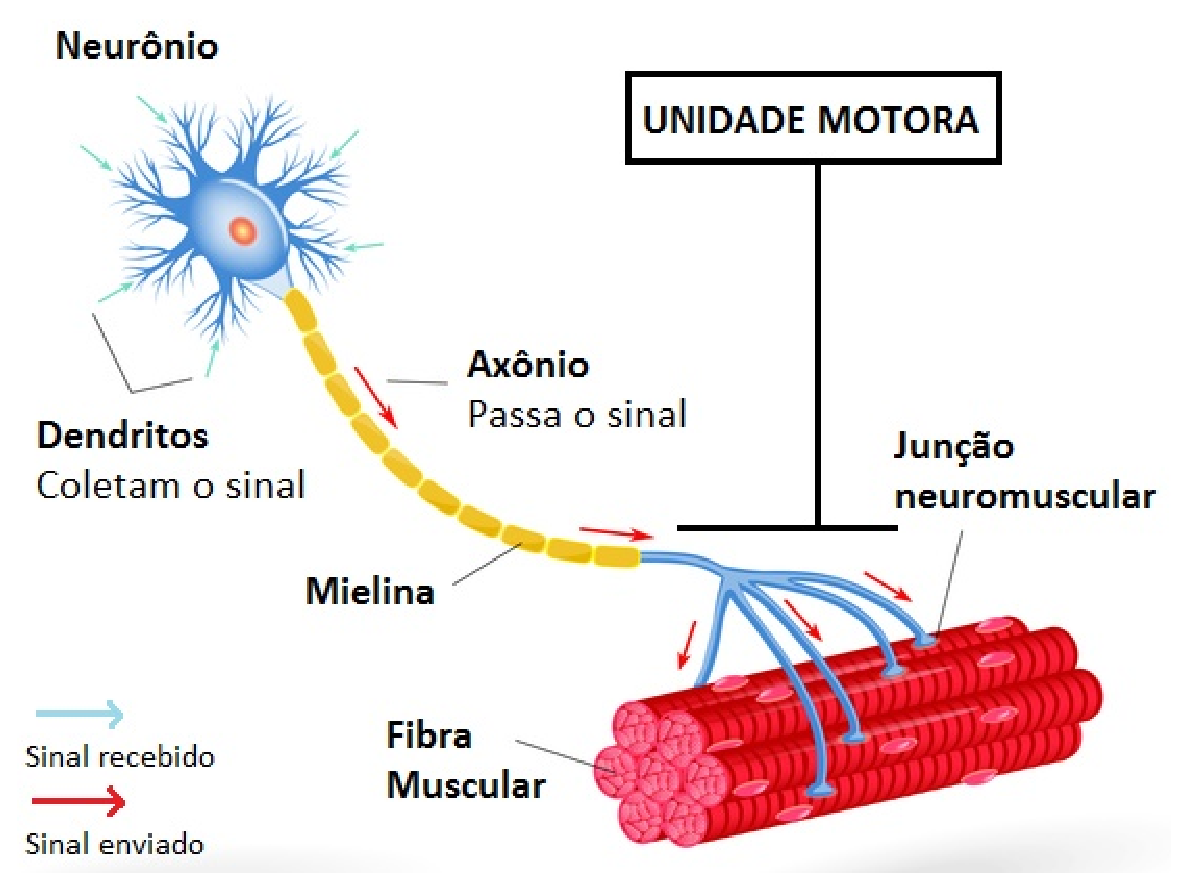
\includegraphics[width=0.8\textwidth]{figuras/motor-neuron.eps}
    \caption{Modelo de uma unidade motora.}
    \label{UnidadeMotora}
\end{figure}

A equação que descreve um sEMG é ~\ref{eq:EMGT}. Um sEMG é a medida ao longo do tempo da contração de um MUP m, de um total de \textit{N, MUPs}, a função n(t) representa possíveis ruídos encontrados na coleta, ambas as funções são parametrizadas pelo tempo \cite{yousefi2014characterizing}.

\begin{equation} \label{eq:EMGT}
    EMG_{t} =\sum_{m=1}^{N} MUPs_{m}(t)+n(t)
\end{equation}

Este tipo de sinal inevitavelmente encontra ruído do equipamento e de outras fontes biológicas presentes no corpo do indivíduo \cite{yousefi2014characterizing}.

Com relação a DP o tremor de repouso é o sintoma mais comum, possuindo uma frequência entre 4 e 6 Hz.
\cite{jankovic2008parkinson}

\section{Usos}
A sEMG é largamente utilizada por pelas diversas áreas científicas que estudam o movimento humano, como Médicos, Fisioterapeutas, Fonoaudiólogos e profissionais em Educação Física\cite{nascimento2012surface}.

\section{sEMG e aprendizado de máquinas}
A utilização de Aprendizado de máquinas em conjunto com sEMG para o auxílio na detecção de alguma doença, já é um tópico bem explorado possuindo diversas publicações relacionadas a esta área de estudo, na base de dados Capes a string de busca '(emg AND (machine learning))' retornou 4.217 resultados, no \textit{ScienceDirect} a mesma \textit{string} retornou 2.396 no \textit{ieeexplore} 169.

Como observado na revisão acadêmica de \cite{yousefi2014characterizing}, os estudos relacionados a sEMG e aprendizado de máquinas são separados em  dois tipos de transtornos neuromusculares Miopatia e Neuropatia, onde Miopatia refere-se a um grupo de patologias que atingem diretamente o tecido muscular sem relação com disfunções do sistema nervoso. Já a Neuropatia, onde encontra-se a doença de Parkinson, é caracterizada por qualquer dano nos nervos envolvidos no controle muscular. Ambos os casos possuem diferenças e similaridades, em resumo segundo \cite{yousefi2014characterizing} as diversas técnicas de Aprendizado de máquinas sobre sEMG, pode-se catalogá-las em três etapas, análise, decomposição e classificação, sendo que não é necessariamente sequencial, podendo ser um processo iterativo.

\subsection{Análise}
O pré-processamento ou análise dos dados é uma das partes mais importantes do processo de aprendizado, essa etapa ocorre apos a coleta dos dados, possuindo alguns objetivos como organizar os dados em conjuntos, identificar possíveis problemas como ruídos ou valores desconhecidos, também é comum utilizar esta etapa para simplesmente aprender mais sobre os modelos plotando gráficos e colhendo mais informações, ou ainda realizar tratamento nos dados como transformações lineares para um conjunto de dados mais simples de ser trabalhado. \cite{batista2003pre}. A figura ~\ref{tremor_i_parkinson} representa o sinal EMG do tremor de intensão do grupo com a doença de Parkinson e a figura ~\ref{tremor_intensao} corresponde ao grupo de controle, estes modelos foram coletados na fase de pré-processamento do projeto.


\begin{figure}[!htb]
   \centering
    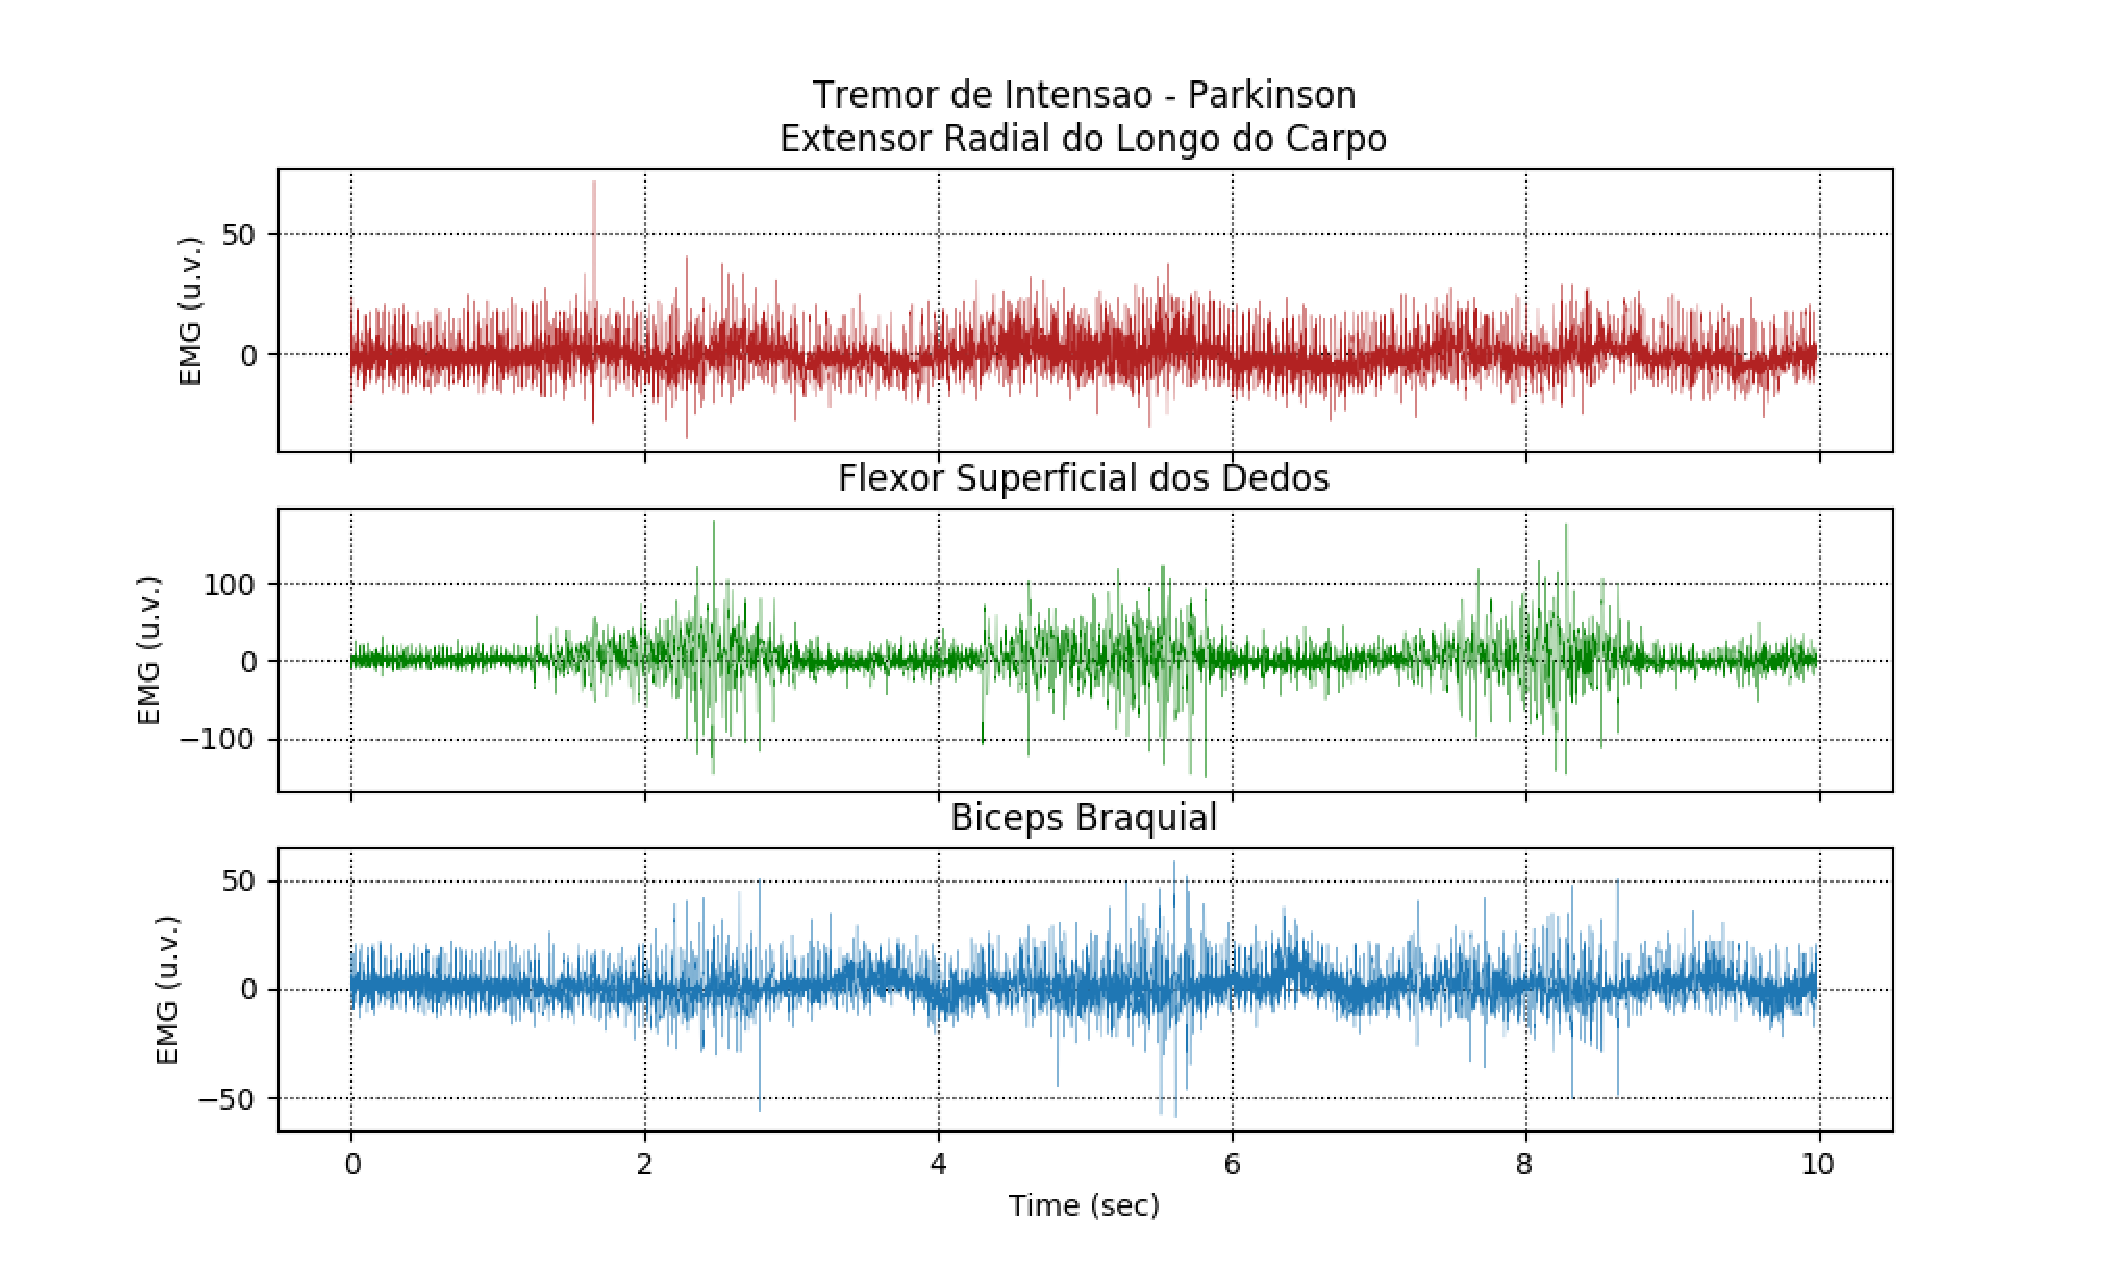
\includegraphics[width=1\textwidth]{figuras/tremor_i_parkinson.eps}
    \caption{PROVISSORIO!!!sEMG do tremor de intensão grupo com a Doença de Parkinson}
    \label{tremor_i_parkinson}
\end{figure}

\begin{figure}[!htb]
   \centering
    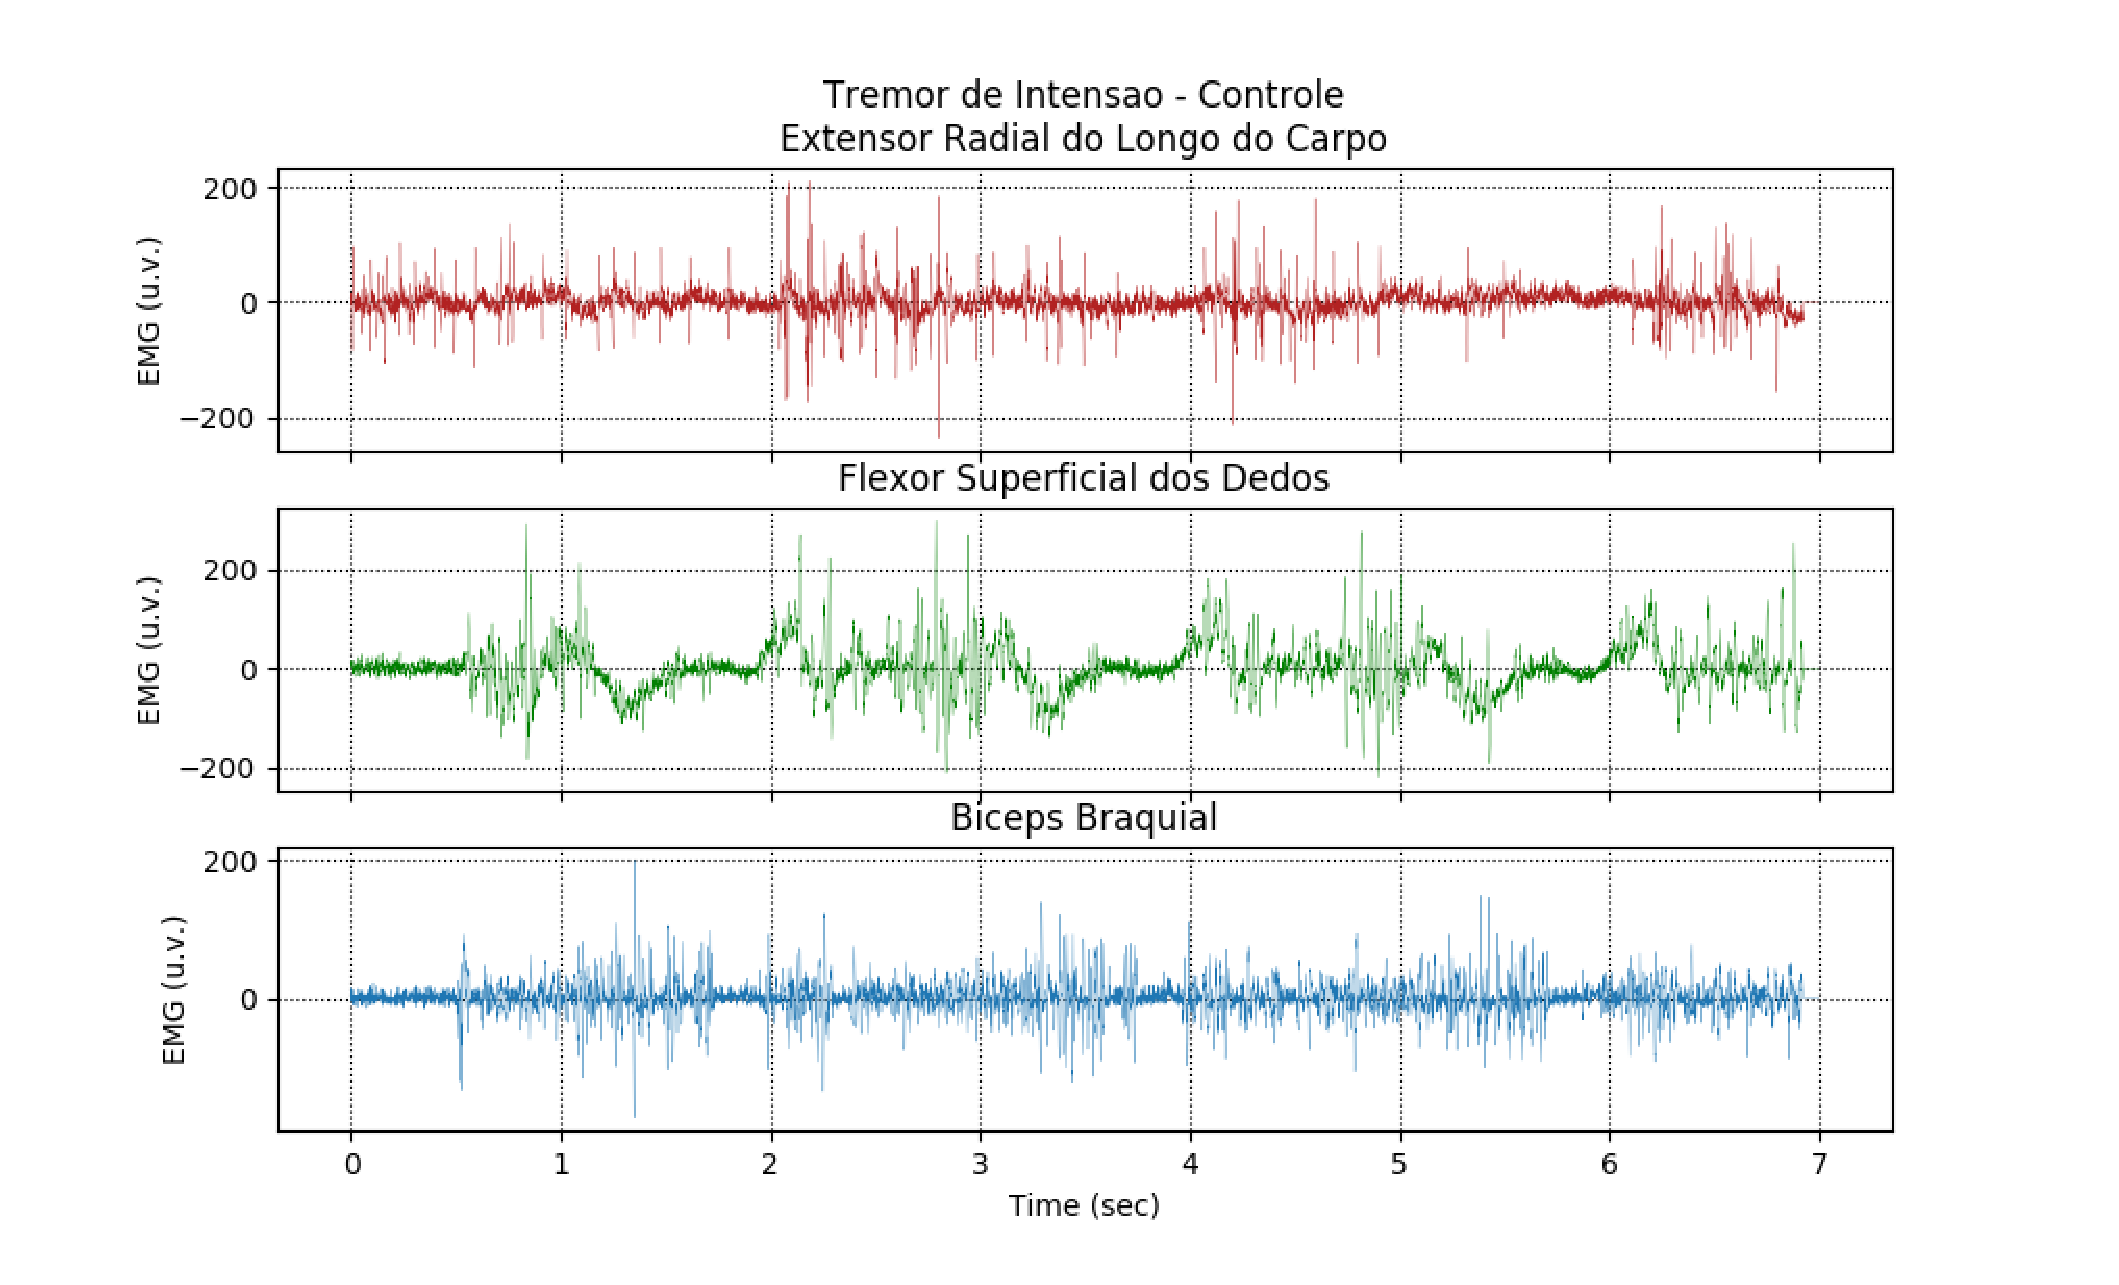
\includegraphics[width=1\textwidth]{figuras/tremor_intensao.eps}
    \caption{PROVISSORIO!!!sEMG do tremor de intensão grupo de controle}
    \label{tremor_intensao}
\end{figure}

\subsection{Decomposição}
Segundo \citeonline{yousefi2014characterizing} a decomposição de um sinal EMG consiste de cinco etapas, aquisição, segmentação, extração de \textit{features}, agrupamento de MUPs e atribuição de MUP.

A seleção das \textit{features} ou características, é a distinção de um sinal bruto em informações úteis, esta informação tratada consiste uma \textit{feature}, a qual será utilizada para treinar o modelo, além disto busca-se remover a parte indesejada do sinal e interferências associadas \cite{phinyomark2012feature}.

Esta etapa deve ser trabalhada cuidadosamente, uma vez que erros podem prejudicar a classificação dos modelos, na pesquisa realizada por \cite{phinyomark2012feature} verificou-se que através de gráficos de dispersão, analise estatística e classificação indicou que a maioria das \textit{features} no domínio do tempo são redundantes e desnecessárias, sendo melhor agrupadas em quatro tipos energia e complexidade, frequência, modelo de previsão e dependência do tempo. O estudo recomendou o uso das seguintes \textit{features}:

\begin{itemize}
    \item MAV: método de informação de energia.
    \item WL: informação de complexidade.
    \item WAMP: informação de frequência.
    \item AR: método de predição.
    \item MAVS: depedência  do tempo.
\end{itemize}

Outro estudo que cita algumas \textit{features} compiladas de outros trabalhos, De acordo com \citeonline{yousefi2014characterizing} as \textit{features} são:
\begin{itemize}
    \item Amplitude pico a pico, relaciona os valores nas extremidades minima e máxima de ativação de uma MUP.
    \item Duração entre inicio e termino de ativação de uma MUP.
    \item Área de uma MUP, é obtida integrando á área resultante da duração do movimento de uma MUP.
\end{itemize}

Um bom resultado na decomposição foi realizado por \cite{yousefi2014characterizing} que realizou uma classificação utilizando o algorítimo SVM, o qual obteve uma acurácia de 70.4\% no modelo, utilizando uma técnica de extração de \textit{feature} \textit{wavelet}, que utiliza uma função capaz de remodelar uma função no domínio do tempo em diferentes escalas de frequência e tempo, após a utilização desta técnica o algorítimo SVM obteve uma acurácia de 99.3\%.

